\begin{figure*}[htbp]
\begin{subfigure}{0.48\textwidth}
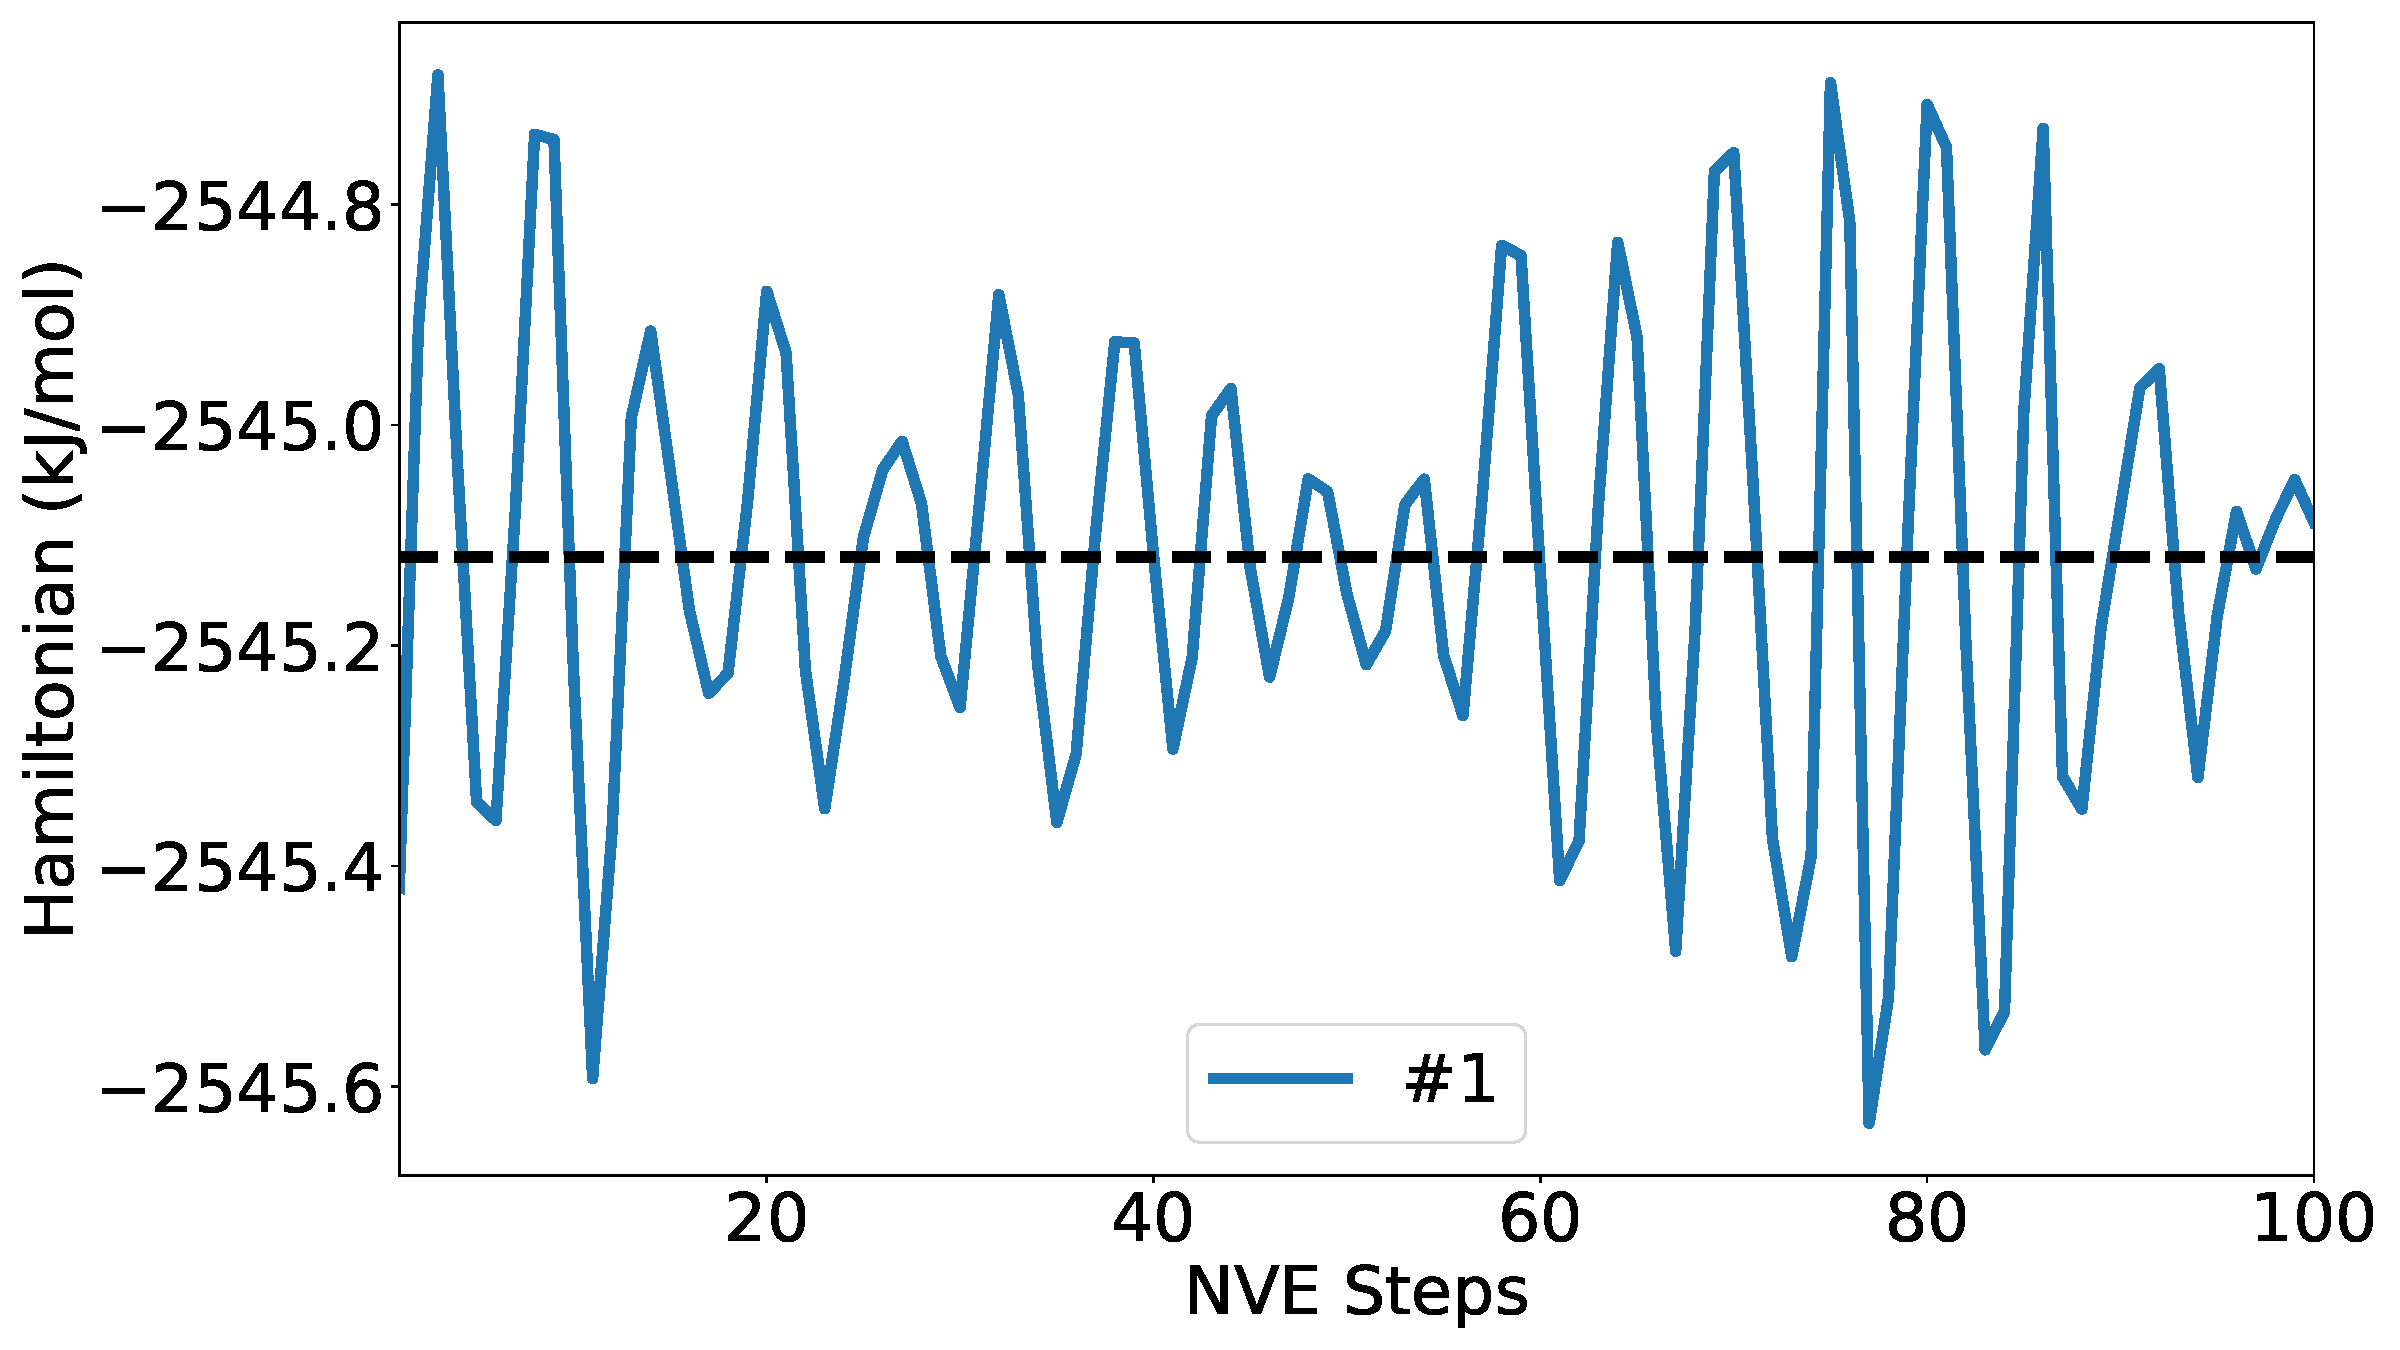
\includegraphics[width=\linewidth]{figs/drift1.pdf}
\end{subfigure}
\begin{subfigure}{0.48\textwidth}
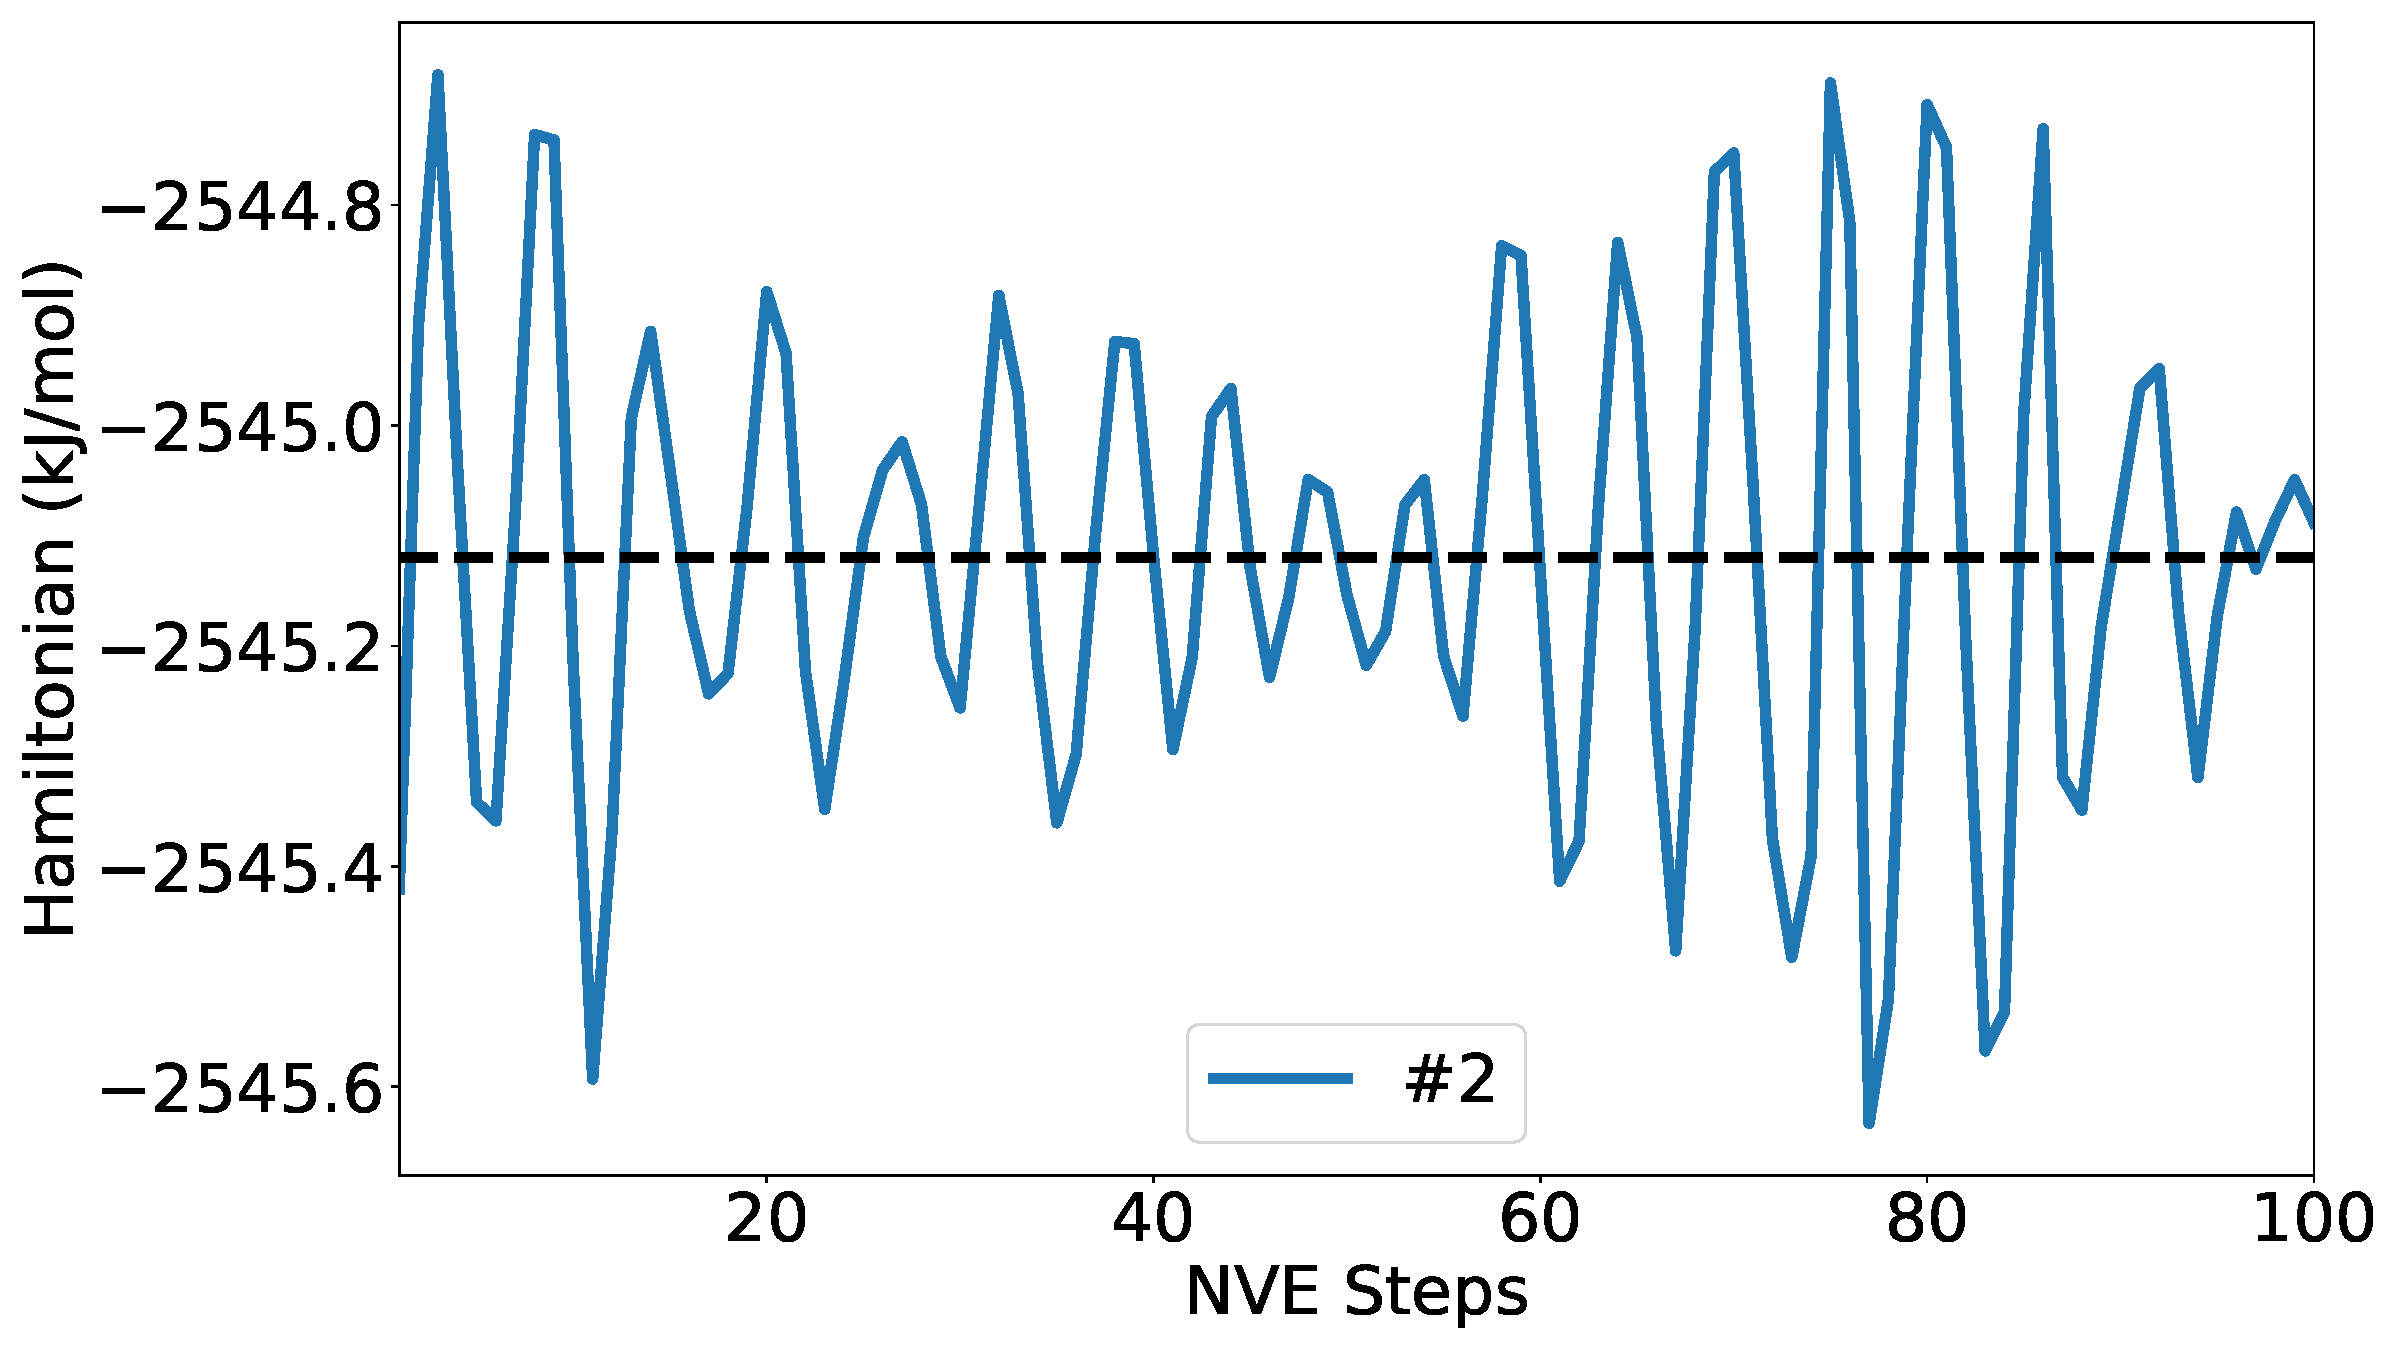
\includegraphics[width=\linewidth]{figs/drift2.pdf}
\end{subfigure}
\\
\begin{subfigure}{0.48\textwidth}
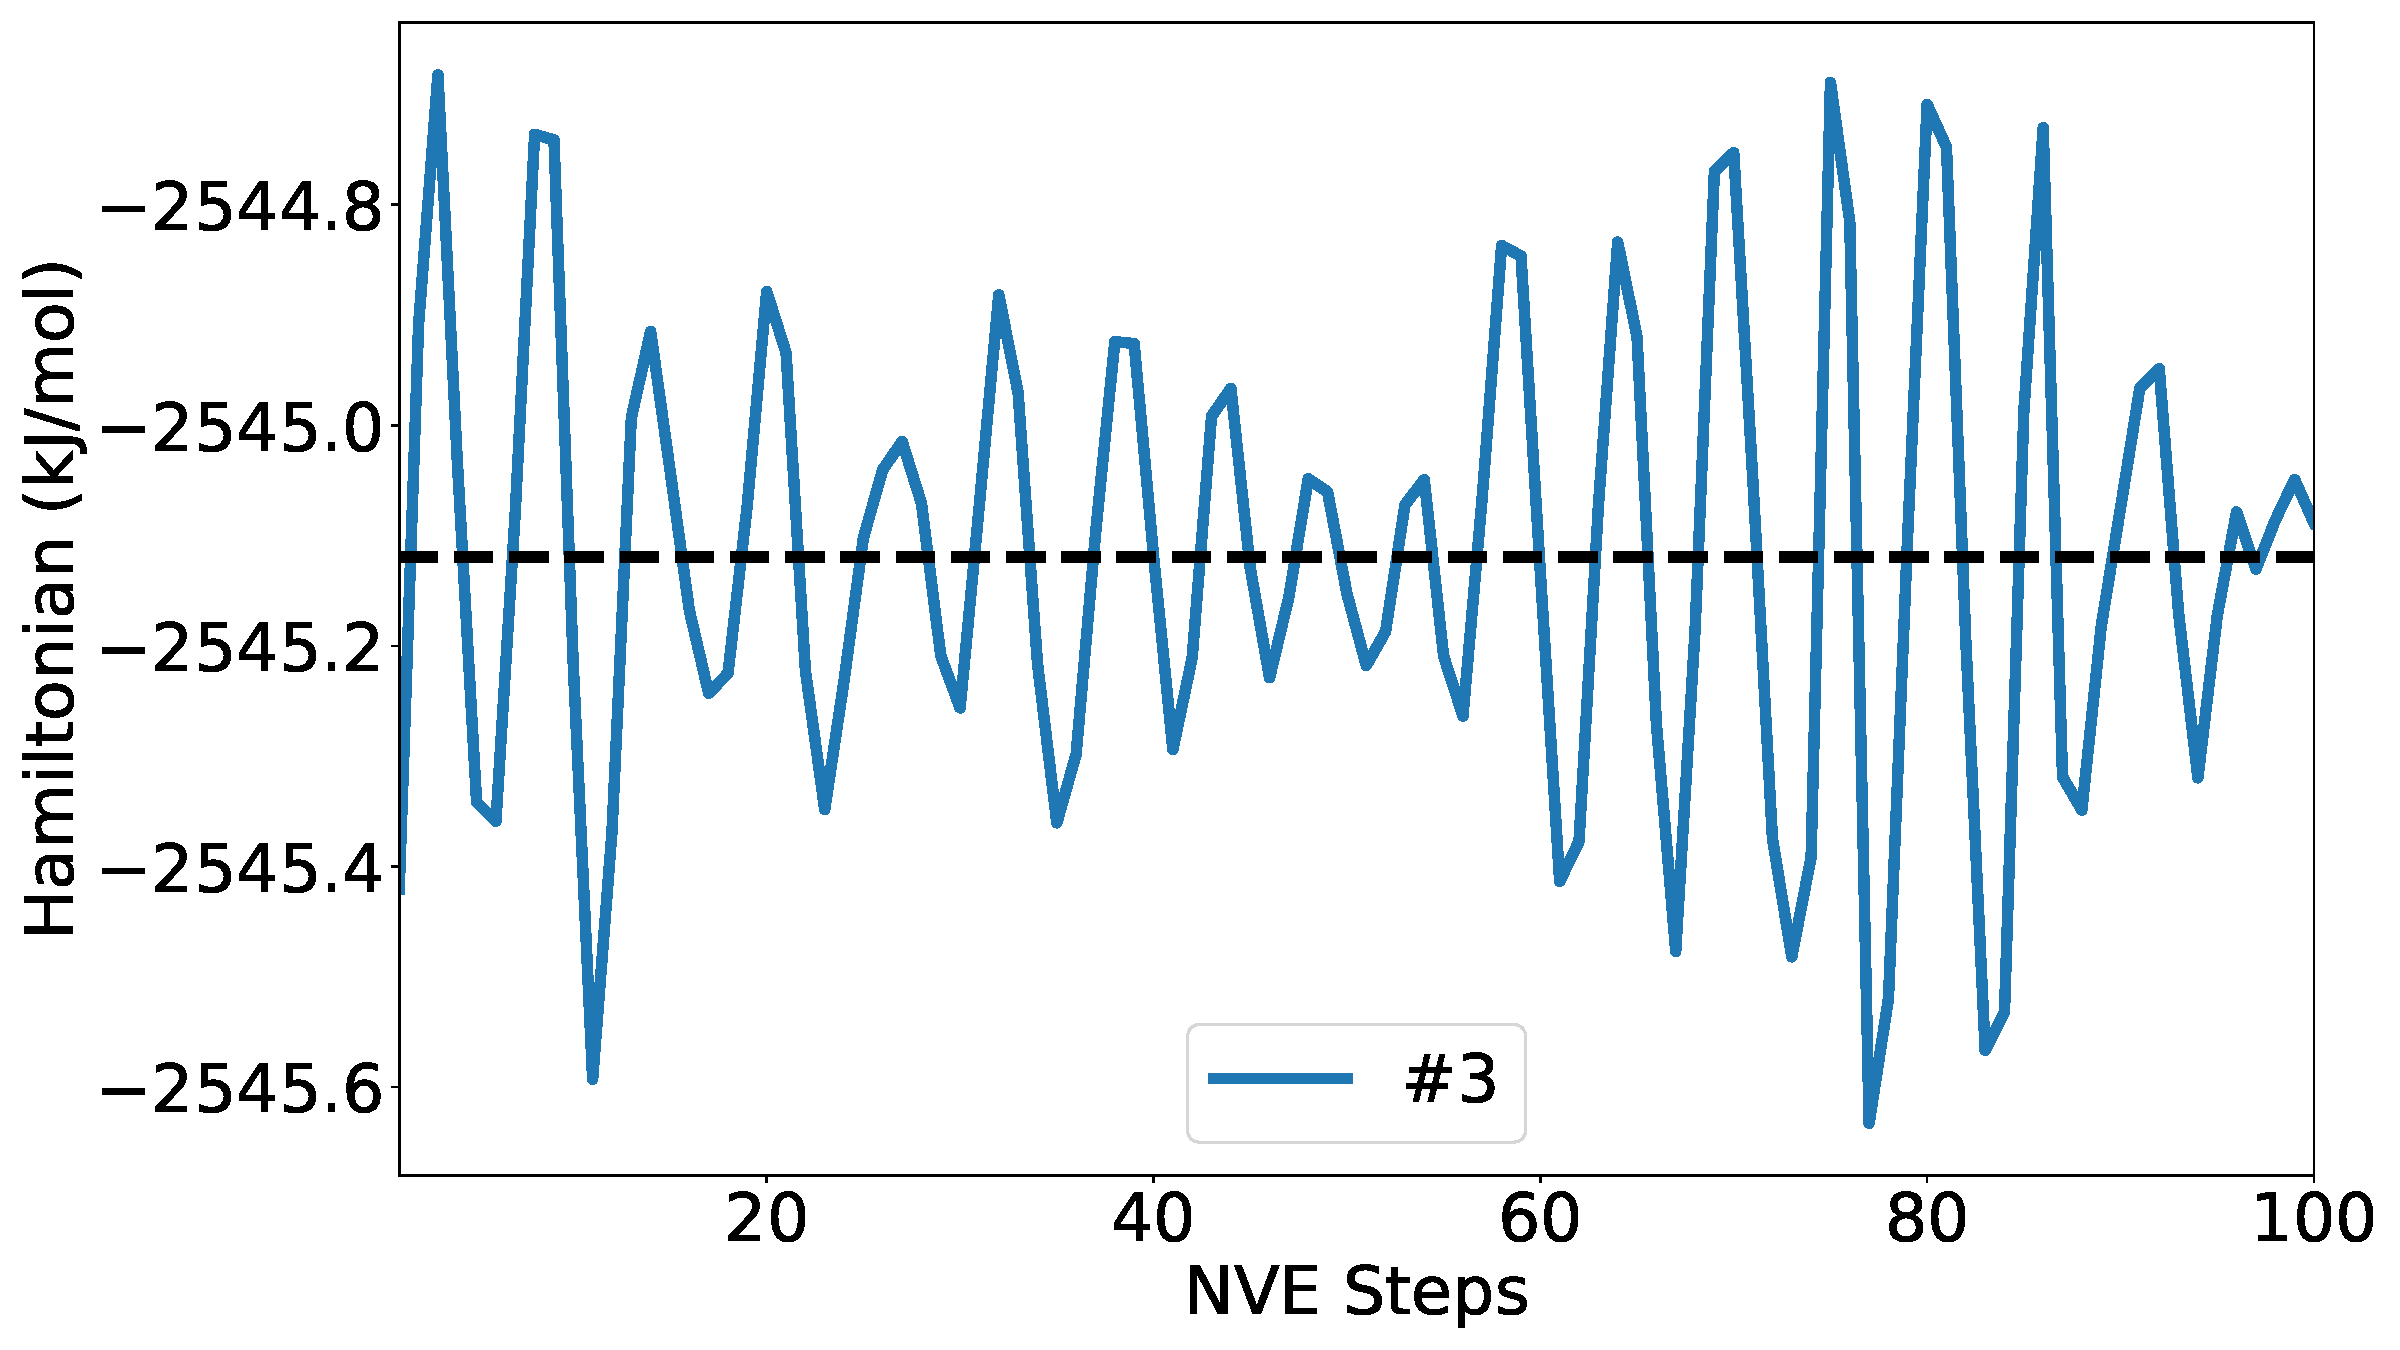
\includegraphics[width=\linewidth]{figs/drift3.pdf}
\end{subfigure}
\begin{subfigure}{0.48\textwidth}
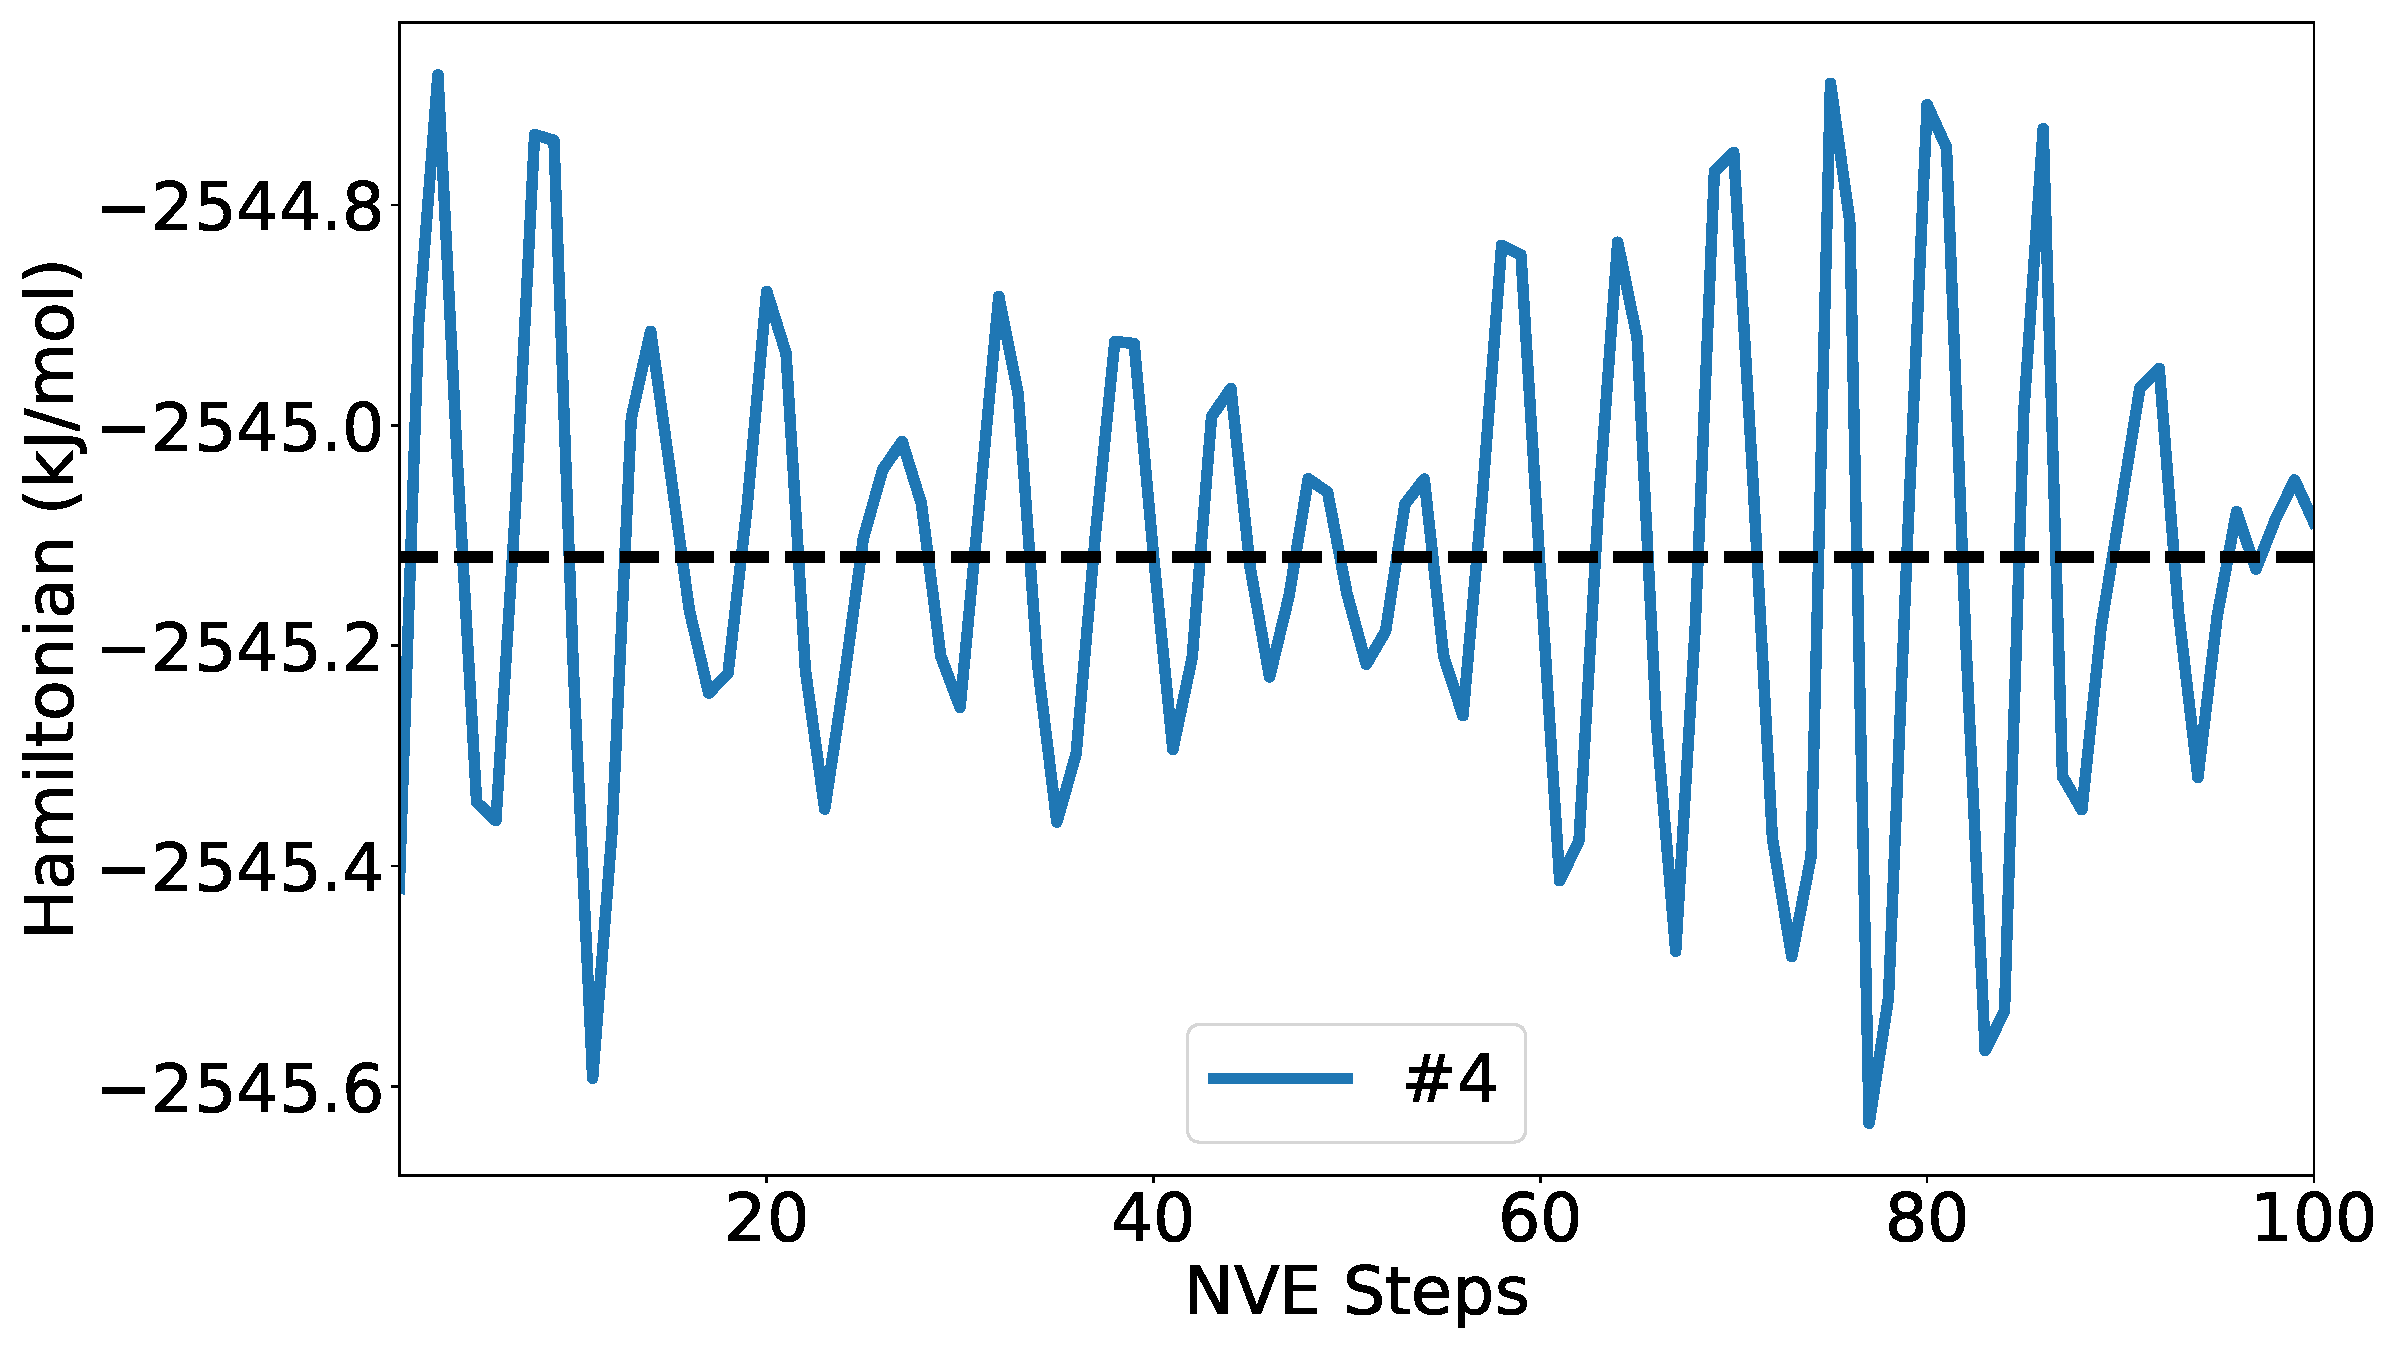
\includegraphics[width=\linewidth]{figs/drift4.pdf}
\end{subfigure}
\\
\begin{subfigure}{0.48\textwidth}
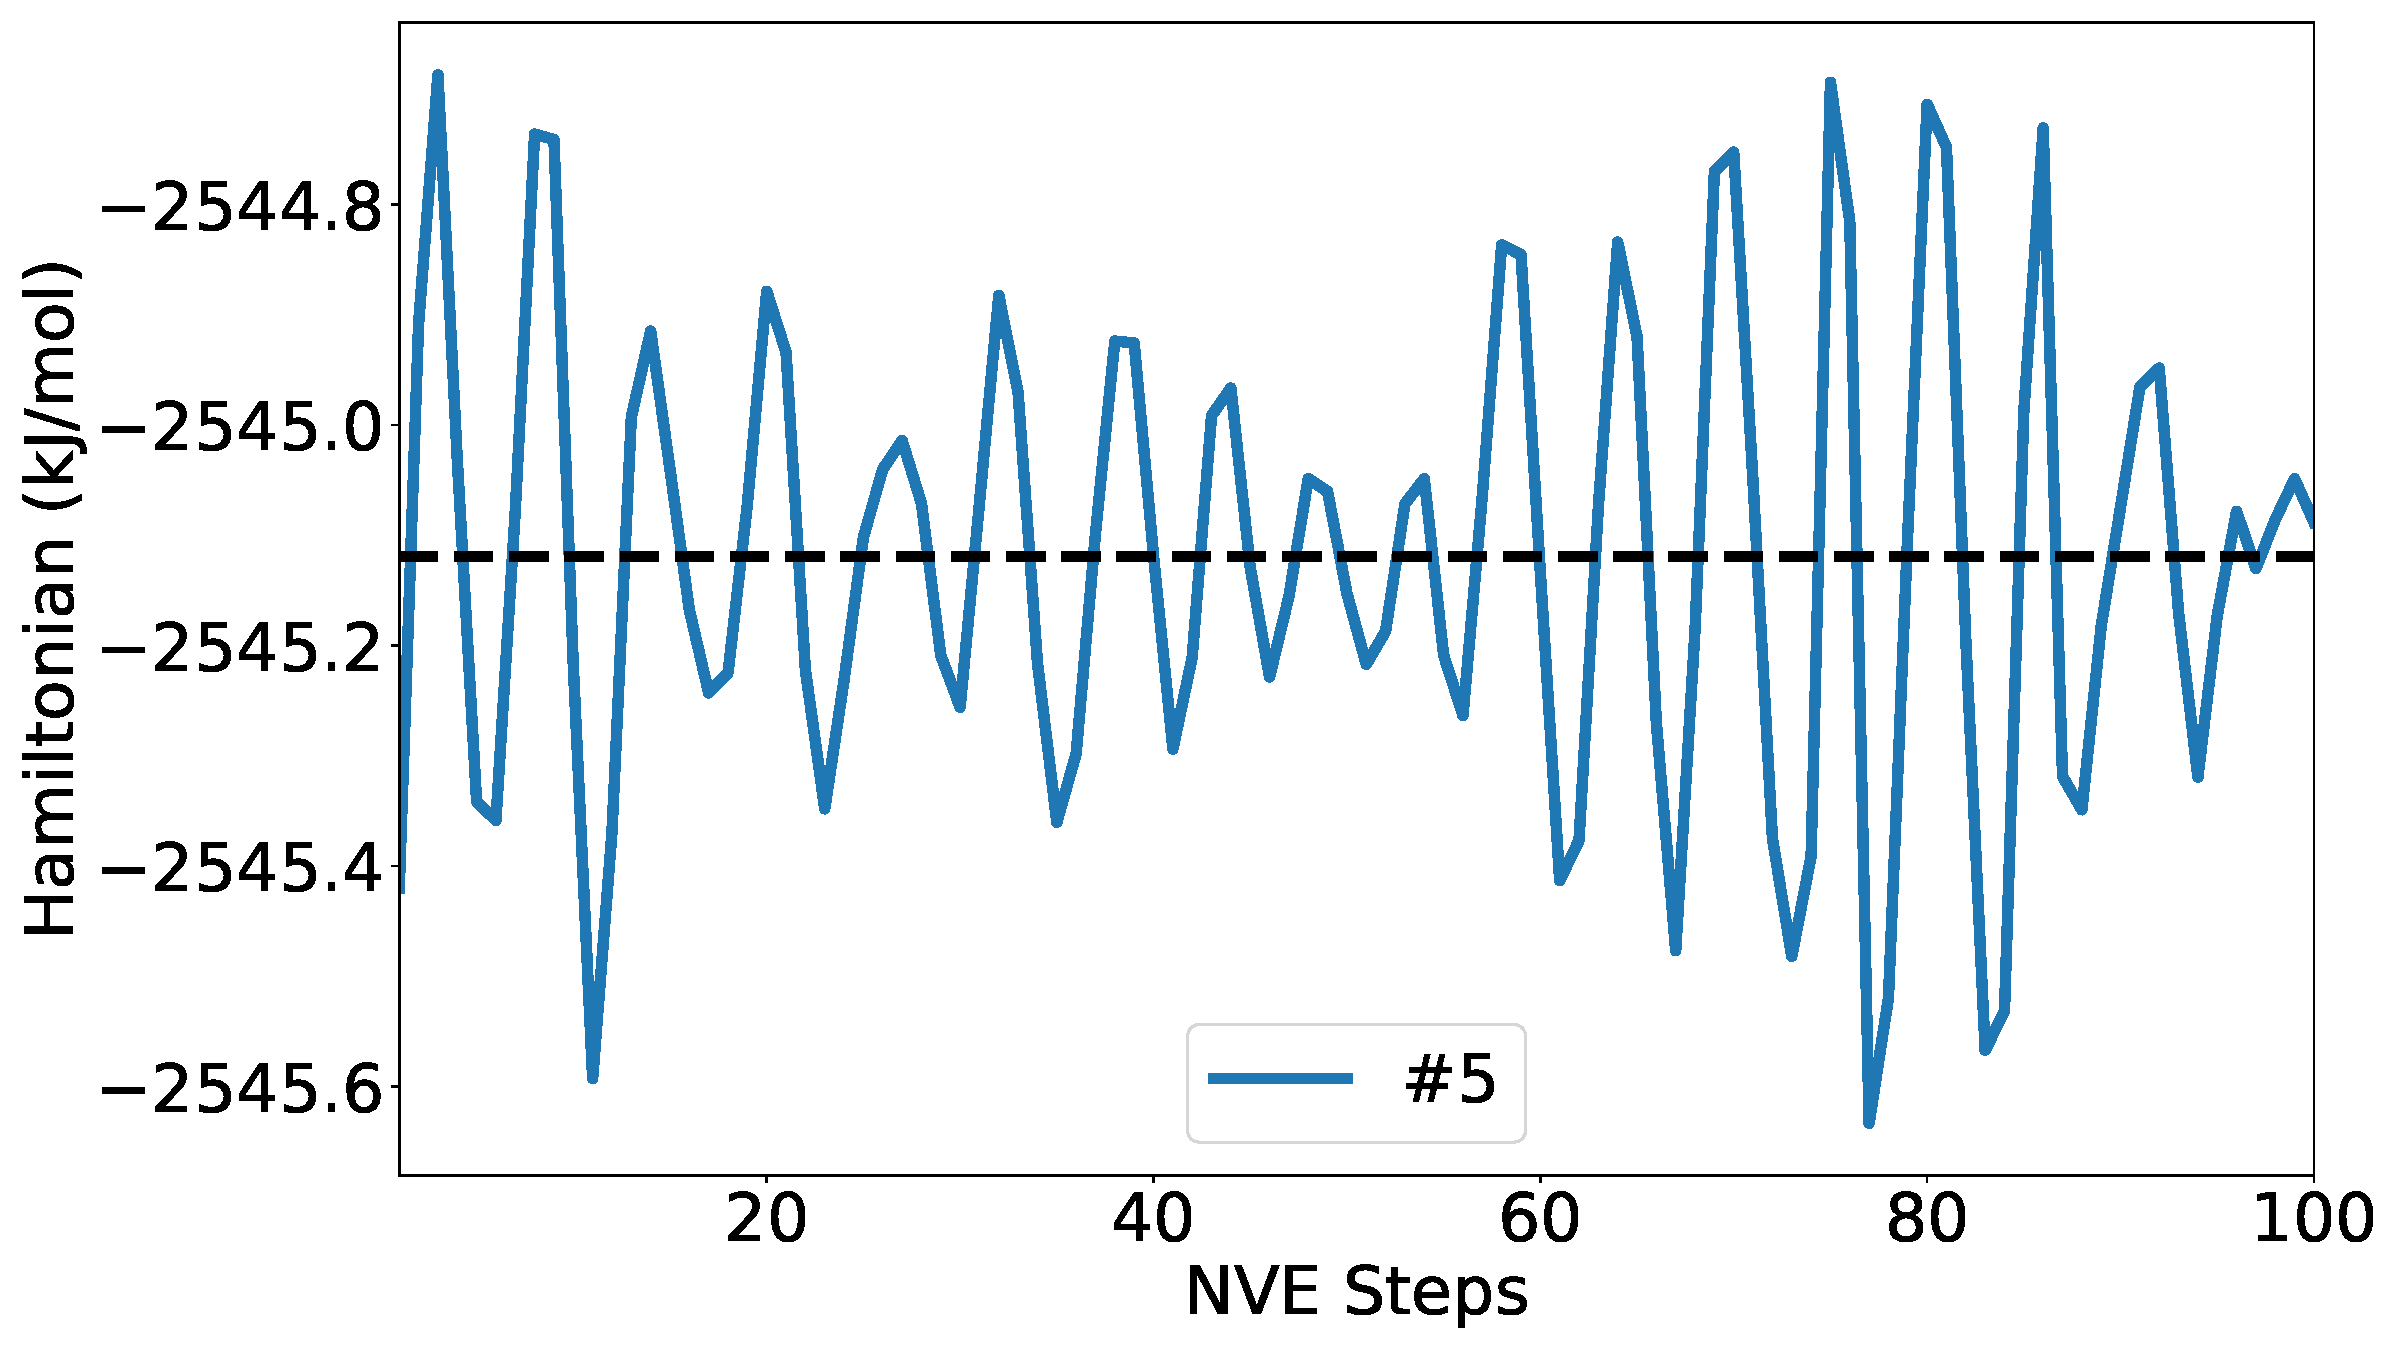
\includegraphics[width=\linewidth]{figs/drift5.pdf}
\end{subfigure}
\begin{subfigure}{0.48\textwidth}
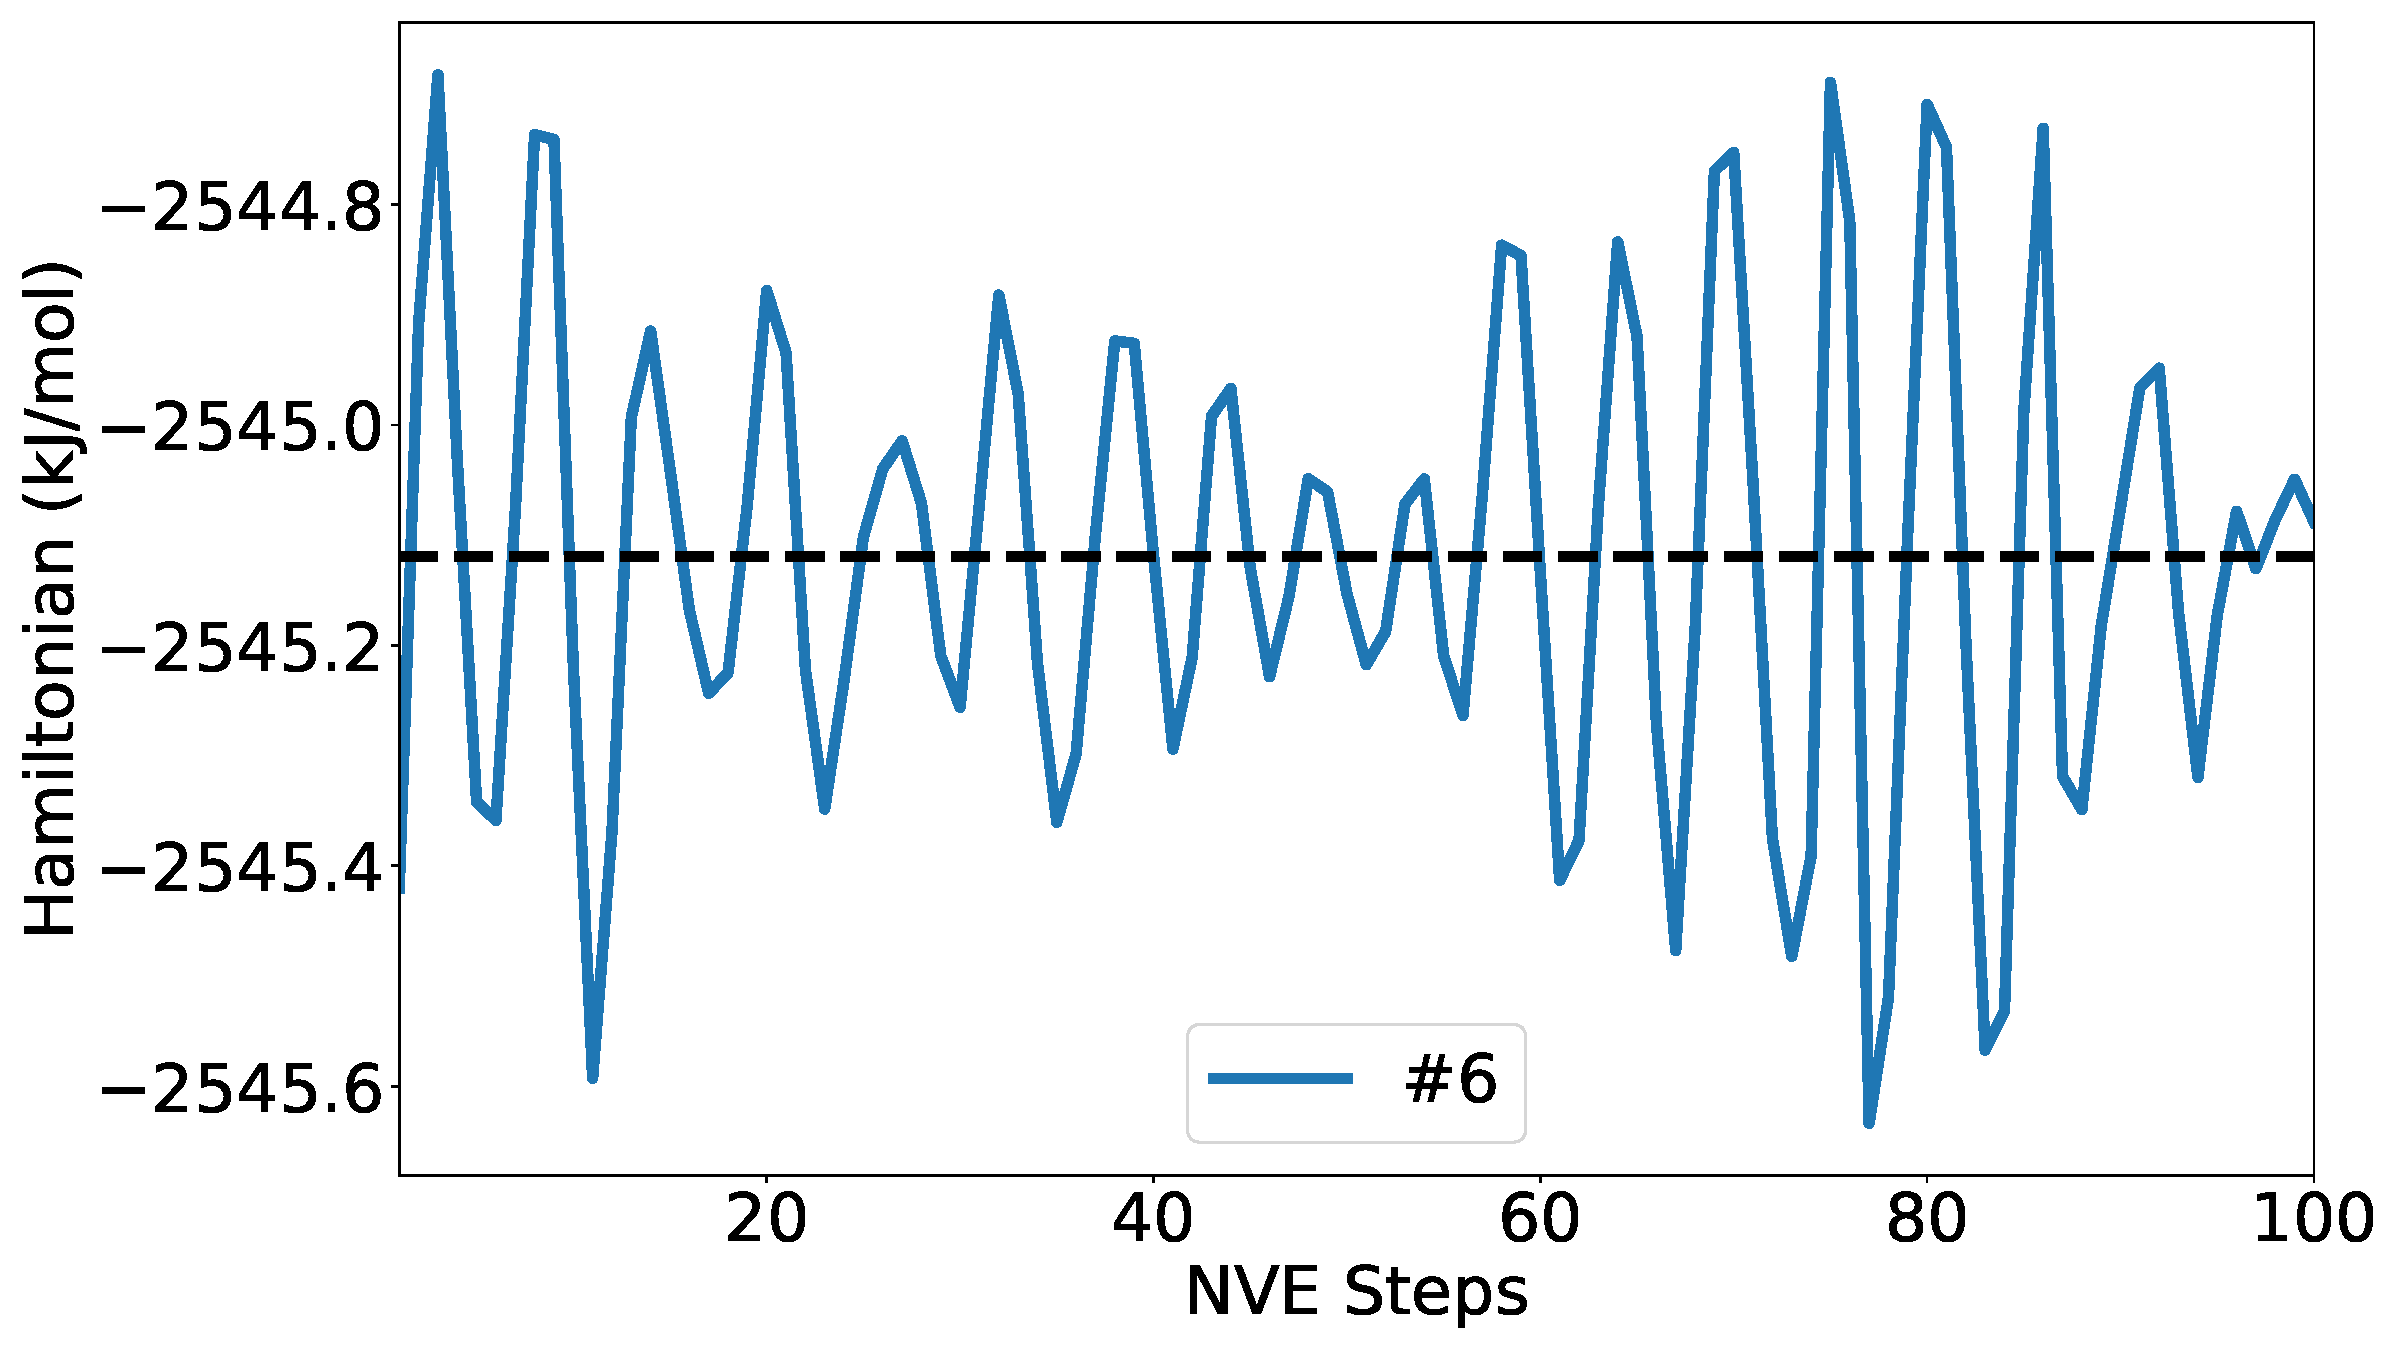
\includegraphics[width=\linewidth]{figs/drift6.pdf}
\end{subfigure}
\\
\begin{subfigure}{0.48\textwidth}
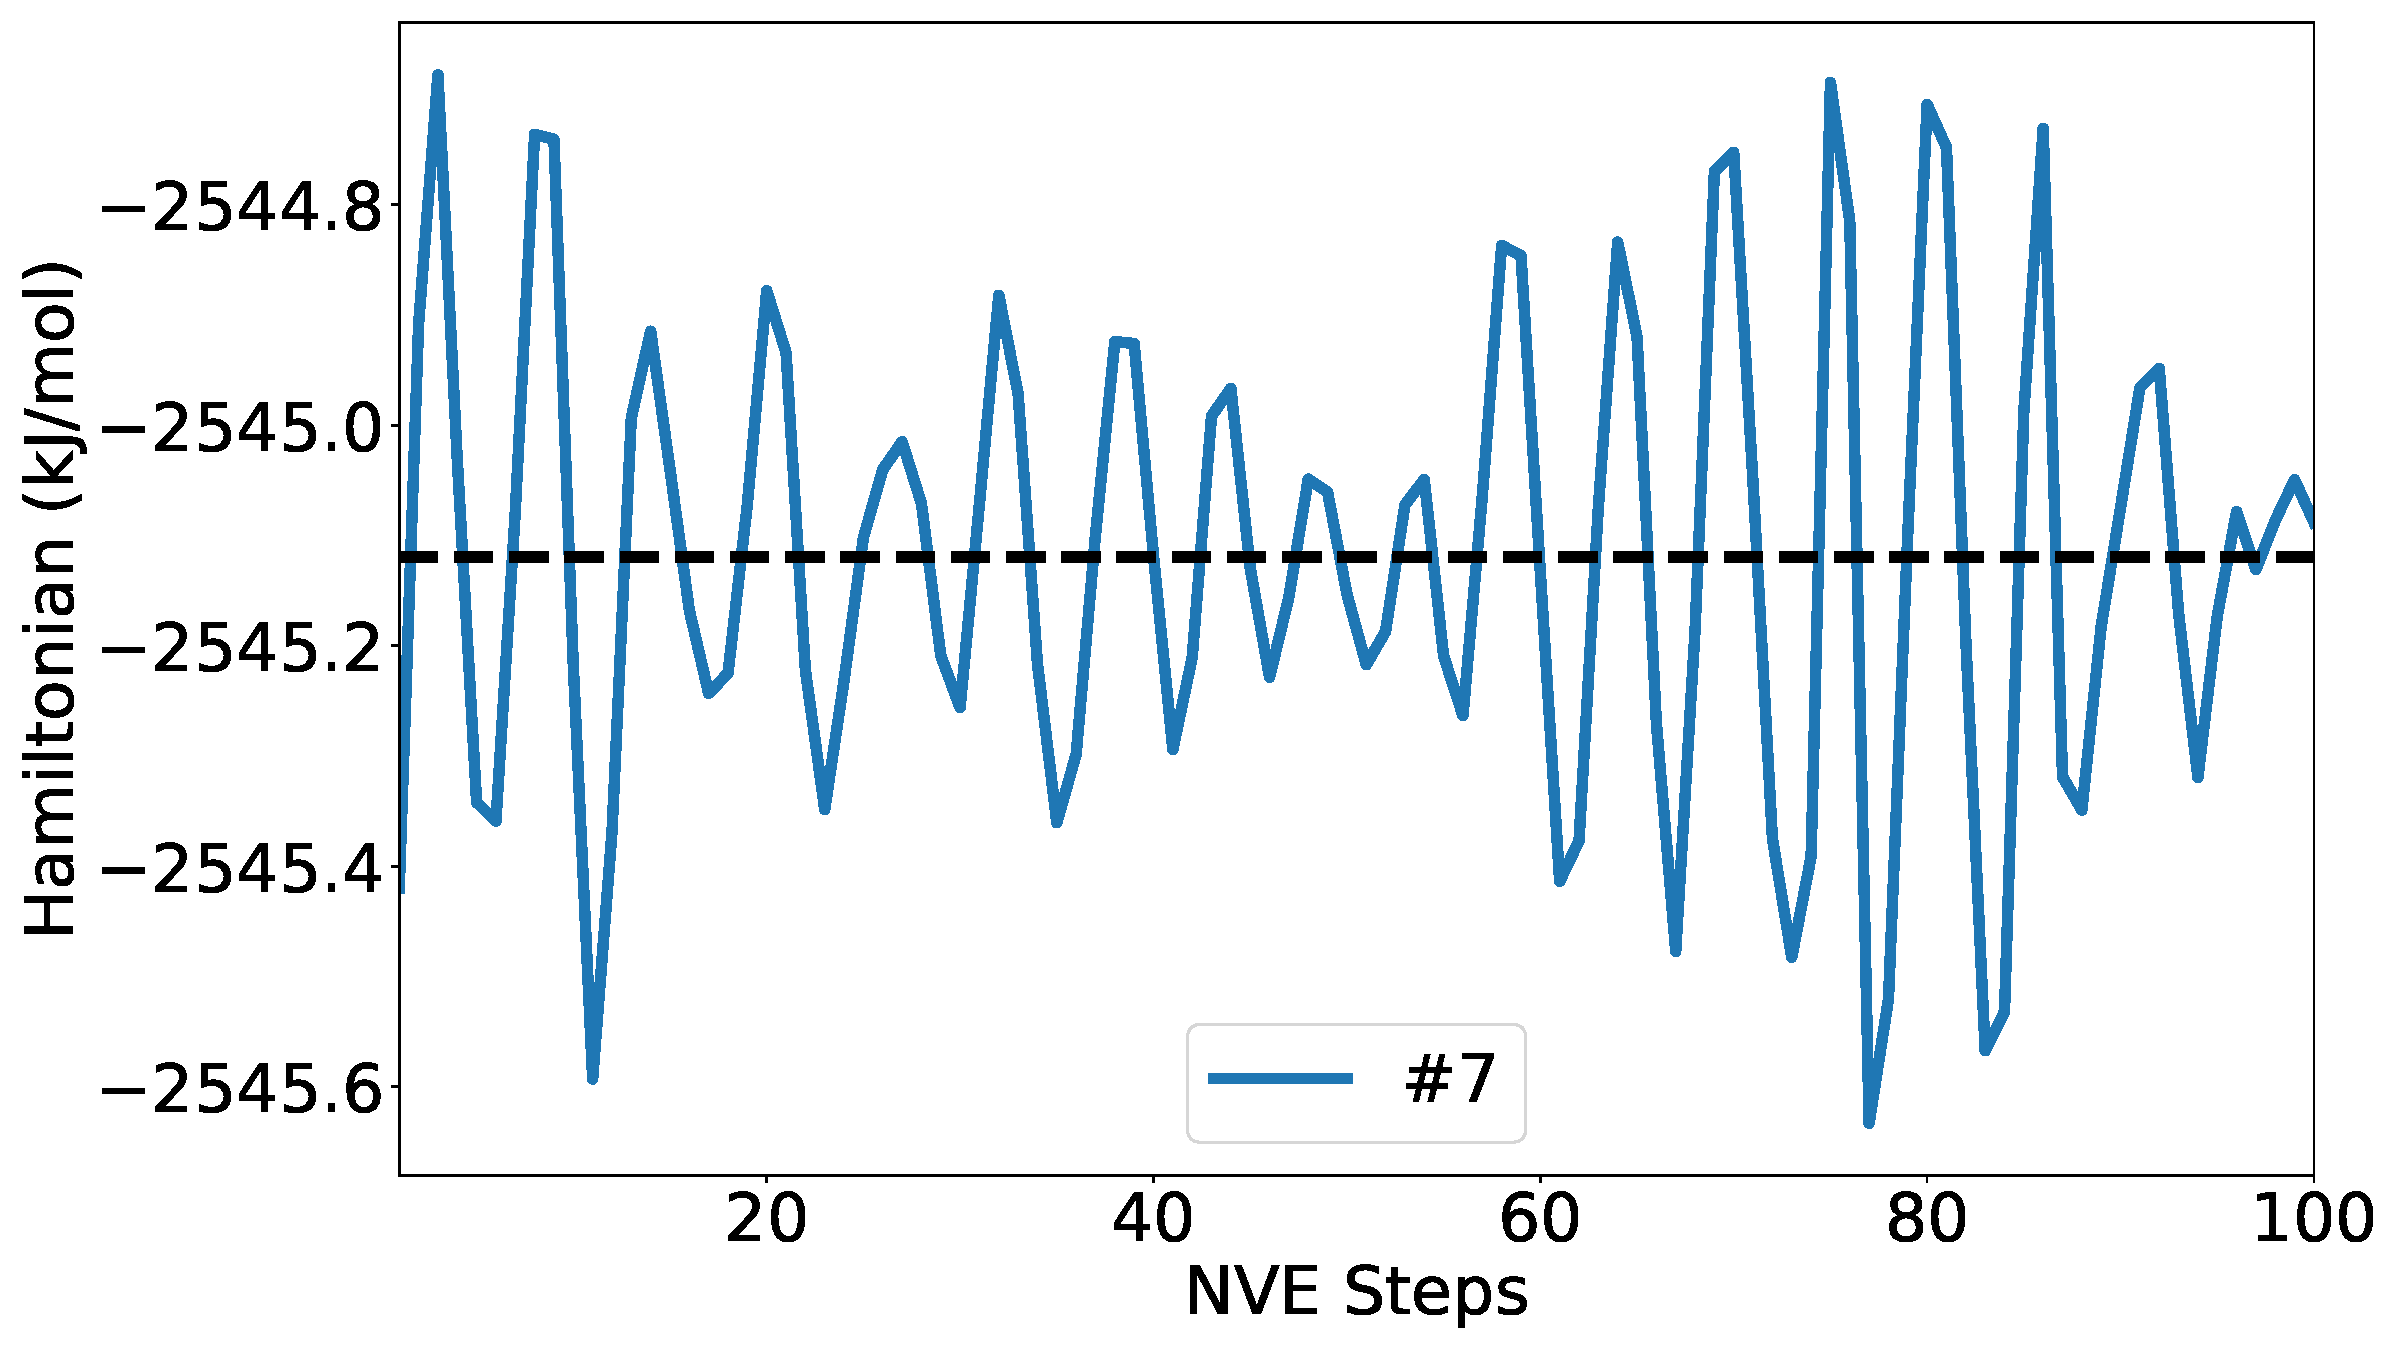
\includegraphics[width=\linewidth]{figs/drift7.pdf}
\end{subfigure}
\begin{subfigure}{0.48\textwidth}
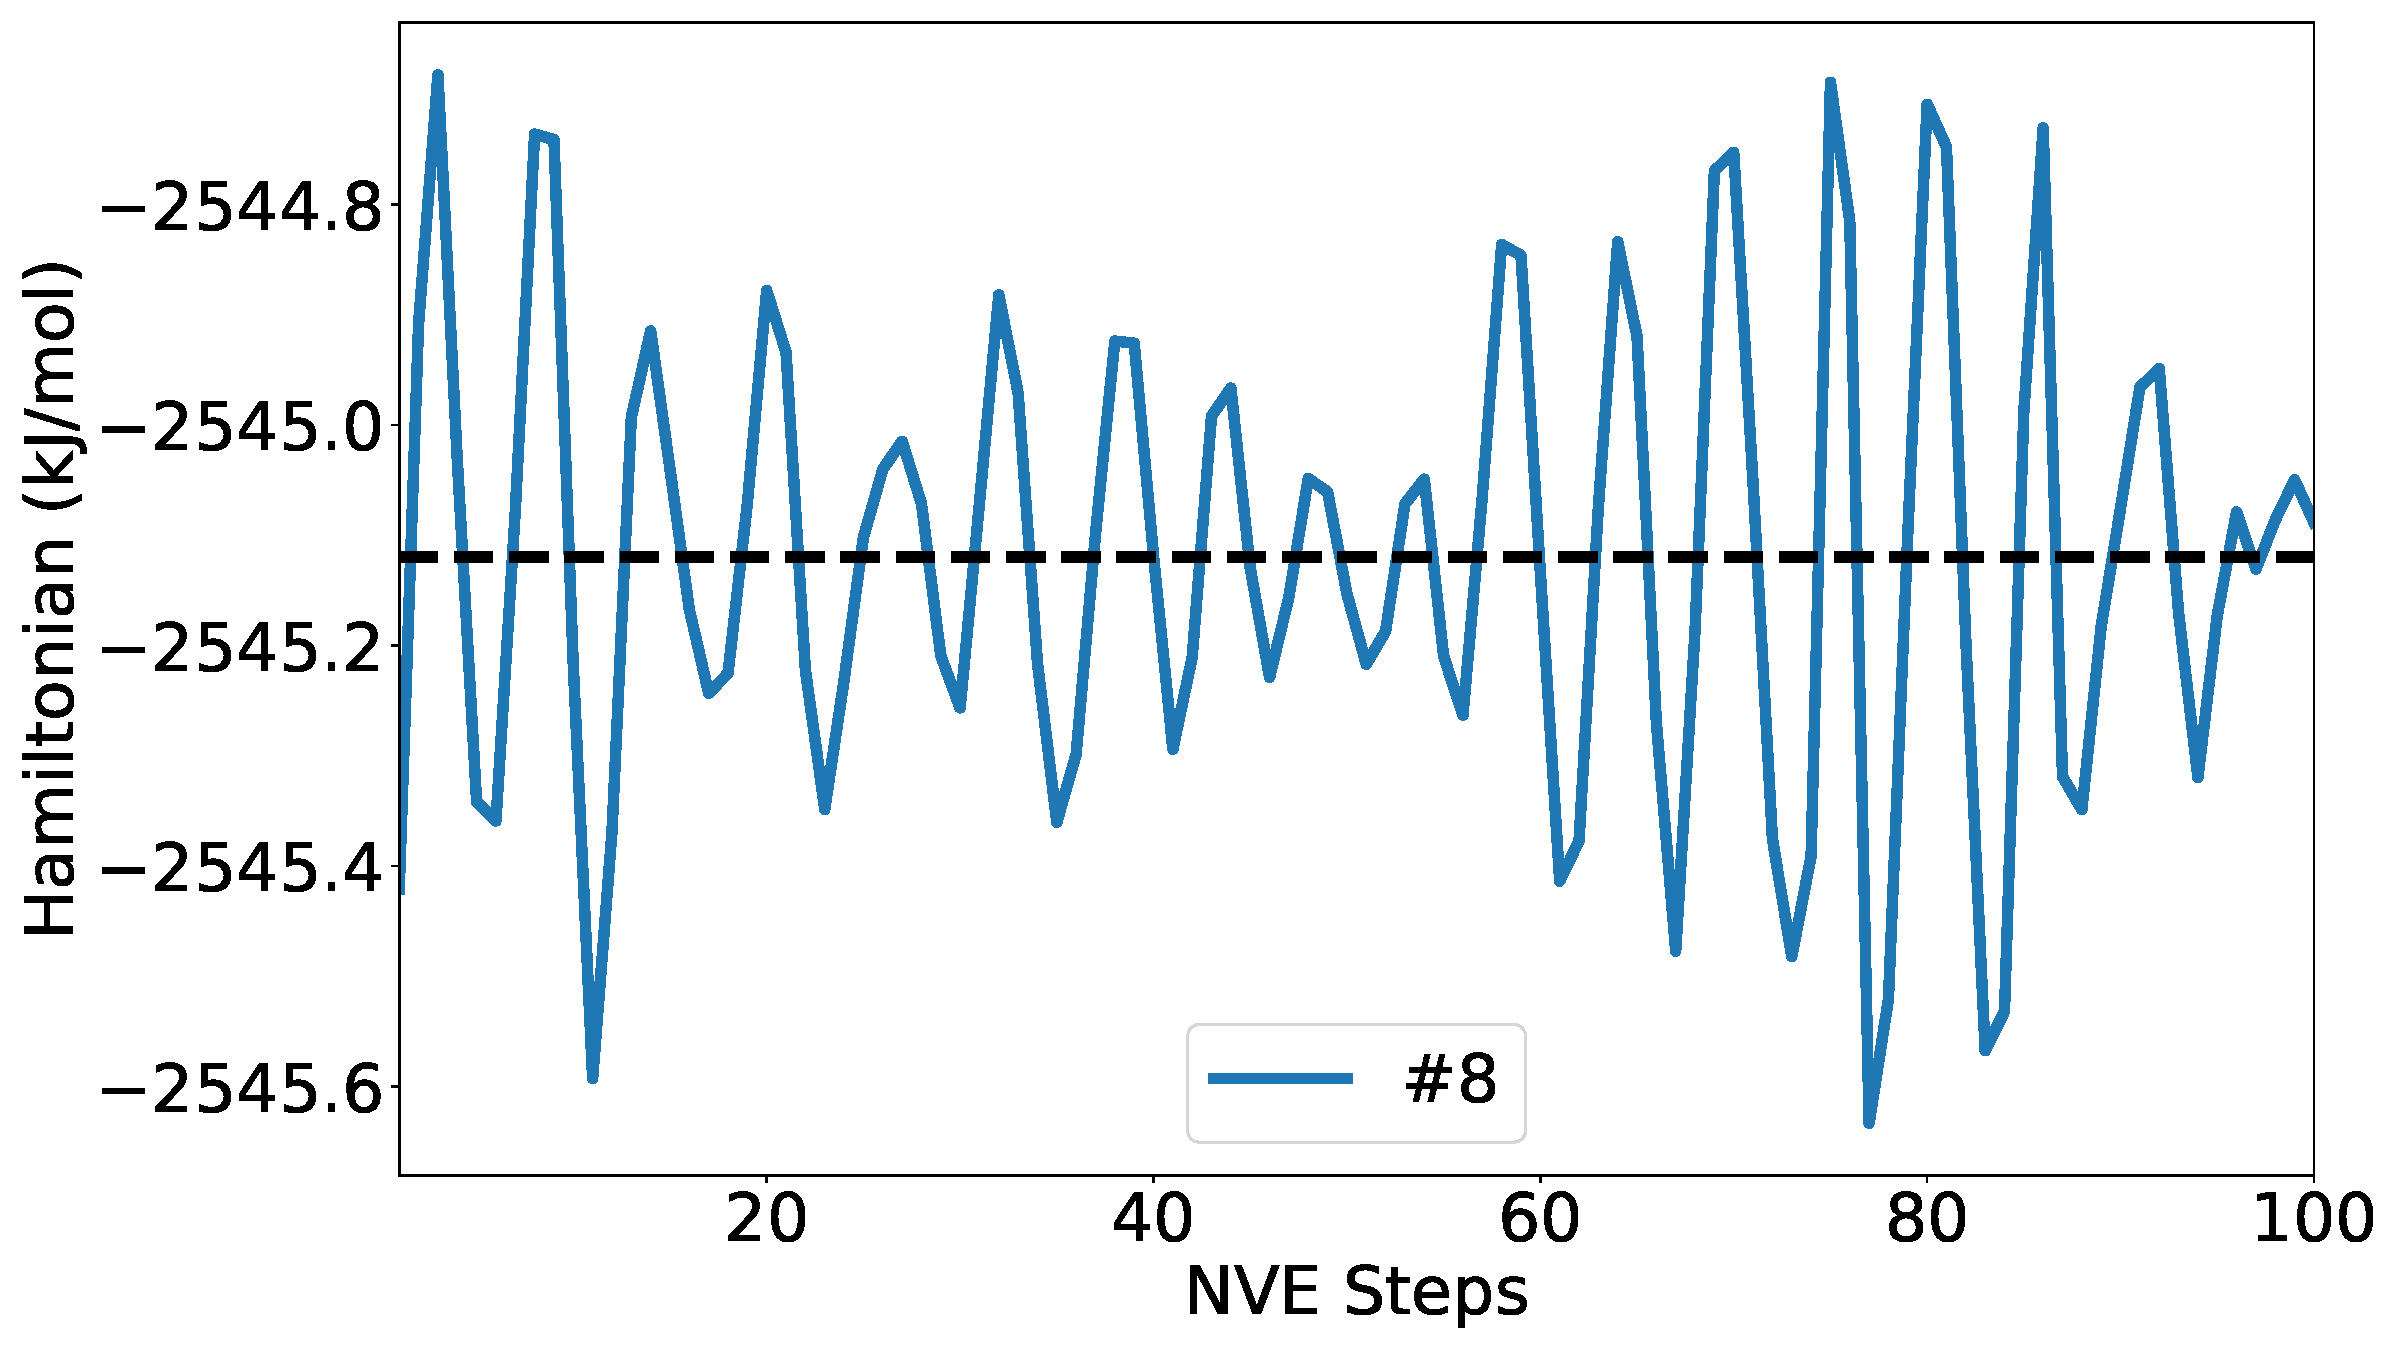
\includegraphics[width=\linewidth]{figs/drift8.pdf}
\end{subfigure}
\caption{Evolution of system Hamiltonians
over 100 time-steps for different deployment strategies.
Each subfigure corresponds to a specific strategy
as detailed in Table~\ref{tb:deploy8}.
Dashed lines indicate the mean Hamiltonian value.}\label{fig:drift}
\end{figure*}
